\setchapterimage[7cm]{ztf/ztf_telescope.png}
\chapter{The Nuclear Sample}\label{ztf}
\labch{nucsam}
Motivated by the three neutrinos coincident with accretion phenomena in the cores of active galaxies, it will be instructive to create a systematic sample of nuclear transients in the ZTF footprint. Furthermore, with the advent of a deep high-cadence sky surveys in the form of the Legacy Survey of Space and Time (LSST, hosted by the Vera C. Rubin Observatory)~\sidecite{Ivezic2019} in the near future, photometric identification of transients will be crucial.

The rate of transients detected by LSST will by far exhaust the available spectroscopic resources, thus requiring informed decisions about when to rely on spectroscopy for classification and characterization. The vast majority of LSST-detected transients will either be photometrically classified, or not classified at all. Therefore, photometrically classifying the ZTF nuclear transients can serve as a precursor study to LSST-era astronomy.

This chapter is dedicate to the nuclear sample, and is structured as follows: A discussion on the sample creation will be followed by different methods to classify the sample. This will be done with a special focus on TDEs.

\section{Sample Creation}
The nuclear sample was created with \texttt{AMPEL} (see Section~\ref{ampel}), using its capability to rerun analyses on archival data. To perform such a rerun, a modified version of the \texttt{AMPEL} nuclear filter was used.

\subsection{\texttt{AMPEL} Nuclear Filter}

The filter is used primarily by the ZTF TDE working group to scan for transient activity that is compatible with an emerging TDE~\cite{Velzen2021a}. In the rerun, it was slightly modified, and used to evaluate each and every alert issued by ZTF.

The logic behind the filtering process can be explained as follows: It selects events with a minimum of photometric quality, ensured by minimum requirements on the number of detections and the brightness. The event at least once needs to pass as `real' (opposed to bogus), and the host needs a high probability of passing as galaxy, not star. Furthermore, \textit{Gaia} is consulted to veto against stars, and the events need to be nuclear, i.e.~happen close to the core of their host galaxy.

\begin{marginfigure}
    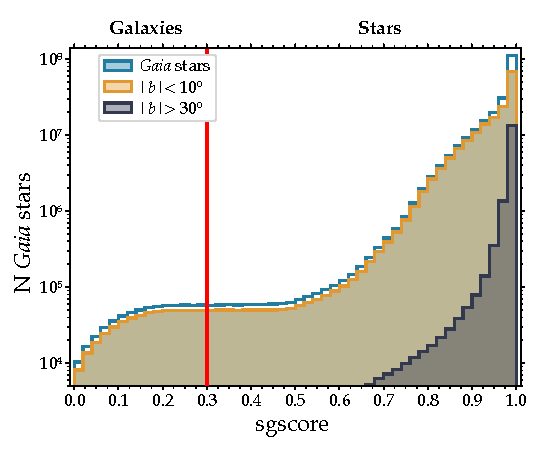
\includegraphics{nuclear/sgscore.pdf}
    \caption[\texttt{sgscore} performance]{\texttt{sgscore} performance evaluated with known \textit{Gaia} stars. At the chosen threshold of 0.3 (red line), the misidentification of stars as galaxies is negligible. Adapted from~\cite{Tachibana2018}}
    \labfig{sgscore}
\end{marginfigure}

The criteria used were:
\begin{description}
    \item[\texttt{sgscore}] As detailed in Section~\ref{ztf_image_subtraction}, \texttt{sgscore} is a machine-learning based star-galaxy score for PS1 objects (low values: galaxy, high values: stars). The transient must at least once have an \texttt{sgsscore} < 0.3 to pass the filter.
    \item[Number of detections] At least 3 detections in both ZTF \textit{g}- and \textit{r}-band are required.
    \item[Galactic cut] The object must be separated by at least \SI{5}{\degree} from the galactic plane to avoid contamination by foreground stars.
    \item[PS1 photometry] To avoid crowded areas, transients where more than 100 objects in the vicinity have a counterpart in PS1 are removed.
    \item[Brightness] At least one alert datapoint of the transient must be brighter than 20 mag.
    \item[\texttt{rbscore}] The real-bogus score separating erroneous detections (low values) from real ones (high values, see Section~\ref{ztf_alerts}) must be larger than 0.3. Note that for more recent data, also \texttt{deep real bogus} is available, which promises vastly better results \sidecite{Duev2019}. Older alerts from 2018 or 2019 do not contain this information, and there is no direct translation from an \texttt{rbscore} threshold to a \texttt{drbscore} threshold. For these reasons and to maximize consistency, we restricted ourselves to using only the older \texttt{rbscore}. The quite loose cut of 0.3 does not entail overly large contamination, as we also require the transient to have a PS1 counterpart. Figure~\ref{fig:rbvsdrb} shows a comparison of the False Negative Rate (FNR) of \texttt{rbscore} vs. \texttt{drbscore}. At the chosen threshold of $0.3$, the FNR for both algorithms is a the percent level.
    \item[Core distance] For all objects that make it this far, their distance to the core is computed. To make this more robust, three different distance metrics are computed. The \textbf{mean distance} to the PS1 source in the reference images, the \textbf{median distance} to that, and lastly, a \textbf{weighted distance}. The latter is computed according to~\sidecite{Velzen2019} and accounts for the fact that the RMS of the angular core distance scales linearly with magnitude. $\sigma_\text{dist}$ = $0.24 + 0.04(m-20)$, where $m$ is the difference photometry magnitude. This stage rejects all transients for which none of the three distances lies below 0.5 arcseconds.
\end{description}

\begin{figure}[htpb]
    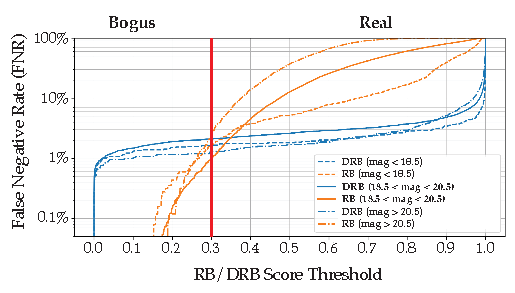
\includegraphics[width=0.9\textwidth]{nuclear/rb_v_drb.pdf}
    \caption[\texttt{rbscore}/\texttt{drbscore} performance]{\texttt{rbscore} vs \texttt{drbscore} performance, evaluated in terms of false negative rate as a function of the threshold. Adapted from~\cite{Duev2019}. The chosen threshold of 0.3 is shown as red vertical line. At that value, \texttt{rbscore} has a False Negative Rate of \SI{\approx1}{\percent} in the relevant magnitude range of $18.5 < \text{mag} < 20.5$.}
    \labfig{rbvsdrb}
\end{figure}

This filter was then applied to all ZTF alerts issued between 1 July, 2018 and 1 January, 2022, comprising 3.5 years of data in total.

\subsection{Rejection Statistics}
From a total sample of XXX alerts issued by ZTF during these 3.5 years, ultimately \textcolor{red}{11687} nuclear transients are selected. The survival rates during the filtering process are shown in Fig.~\ref{fig:nuclear_decision}, with complete alert stream on top, different thematically grouped rejection stages in between and the final accepted alerts on the bottom.

\begin{figure}[h!]
    \begin{tikzpicture}[node distance=1.2cm]
        \node (start) [keep] {XXX initial ZTF alerts};
        \node (dec1) [decision,  font=\small, align=center, below of=start] {SQL\\Filter};
        \node (expl1) [explain, font=\small, align=left, left of=dec1, xshift=-1.8cm] {$<20$ mag\\\texttt{rbscore} $>0.3$\\PS1 dist $<0.5$ arcsec\\$\geq 3$ detections};
        \node (disc1) [discard, font=\small, right of=dec1, xshift=2.1cm] {Discard xx alerts};
        \node (keep1) [keep, font=\small, below of=dec1] {Keep 94,714,866 alerts};
        \node (dec2) [decision, font=\small, align=center, below of=keep1] {\texttt{sgscore}\\veto};
        \node (expl2) [explain, font=\small, align=left, left of=dec2, xshift=-2.2cm] {\texttt{sgscore} $\leq0.3$};
        \node (disc2) [discard, font=\small, right of=dec2, xshift=2.3cm] {Discard 94,485,886 alerts};
        \node (keep2) [keep, font=\small, below of=dec2] {Keep xx alerts};
        \node (dec3) [decision, font=\small, align=center, below of=keep2] {PS1\\veto};
        \node (expl3) [explain, font=\small, align=left, left of=dec3, xshift=-1.5cm] {PS1 source faint enough\\good PS1 photometry};
        \node (disc3) [discard, font=\small, right of=dec3, xshift=2cm] {Discard xx alerts};
        \node (keep3) [keep, font=\small, below of=dec3] {Keep xx alerts};
        \node (dec4) [decision, font=\small, align=center, below of=keep3] {Photometry\\veto};
        \node (expl4) [explain, font=\small, align=left, left of=dec4, xshift=-1.5cm] {$<20$ mag\\$\geq$ 3 detections\\flux increase $>2.5$ mag};
        \node (disc4) [discard, font=\small, right of=dec4, xshift=2cm] {Discard xx alerts};
        \node (keep4) [keep, font=\small, below of=dec4] {Keep xx alerts};
        \node (dec5) [decision, font=\small, align=center, below of=keep4] {Position\\veto};
        \node (expl5) [explain, font=\small, align=left, left of=dec5, xshift=-1.5cm] {$>5$ deg from gal. plane\\not potential mover};
        \node (disc5) [discard, font=\small, right of=dec5, xshift=2cm] {Discard xx alerts};
        \node (keep5) [keep, font=\small, below of=dec5] {Keep xx alerts};
        \node (dec6) [decision, font=\small, align=center, below of=keep5] {\textit{Gaia}\\veto};
        \node (expl6) [explain, font=\small, align=left, left of=dec6, xshift=-1.5cm] {No match to \textit{Gaia} star\\$\leq30$ \textit{Gaia} stars close by};
        \node (disc6) [discard, font=\small, right of=dec6, xshift=2cm] {Discard xx alerts};
        \node (keep6) [keep, font=\small, below of=dec6] {Keep xx alerts};
        \draw [arrow] (start) -- (dec1);
        \draw [arrow] (keep1) -- (dec2);
        \draw [arrow] (dec1) -- node[midway,above] {\small no} (disc1);
        \draw [arrow] (dec1) -- node[midway,left] {\small yes} (keep1);
        \draw [arrow] (dec2) -- node[midway,above] {\small no} (disc2);
        \draw [arrow] (dec2) -- node[midway,left] {\small yes} (keep2);
        \draw [arrow] (keep2) -- (dec3);
        \draw [arrow] (dec3) -- node[midway,above] {\small no} (disc3);
        \draw [arrow] (dec3) -- node[midway,left] {\small yes} (keep3);
        \draw [arrow] (keep3) -- (dec4);
        \draw [arrow] (dec4) -- node[midway,above] {\small no} (disc4);
        \draw [arrow] (dec4) -- node[midway,left] {\small yes} (keep4);
        \draw [arrow] (keep4) -- (dec5);
        \draw [arrow] (dec5) -- node[midway,above] {\small no} (disc5);
        \draw [arrow] (dec5) -- node[midway,left] {\small yes} (keep5);
        \draw [arrow] (keep5) -- (dec6);
        \draw [arrow] (dec6) -- node[midway,above] {\small no} (disc6);
        \draw [arrow] (dec6) -- node[midway,left] {\small yes} (keep6);
    \end{tikzpicture}
    \caption[Nuclear filter flow chart]{Flow chart showing the workings of the nuclear filter.}
    \labfig{nuclear_decision}
\end{figure}

As one can see, the vast majority of alerts are rejected based on them being either too faint, likely being bogus, or likely being stars.

\subsection{Forced photometry}
To be sensitive to early and late-time light curve evolution, forced photometry was acquired for all 11687 transients making the final cut. This was again done with \texttt{fpbot}, see Section \ref{fpbot} for details. The process proved cumbersome due to the enormous data volume (several hunders of GB) that was required to be transferred from IPAC and stored in batches due to computing center restrictions.

\subsection{Infrared Data}
Motivated by the strong dust echo detected for AT2019dsg, AT2019fdr and AT2019aalc, the optical forced photometry dataset was completed with infrared light curves from the \textit{WISE} mission. This was achieved by using the \texttt{timewise} package~\sidecite{Necker2023a} to download all datapoints available for each source location in the \textit{W1}- and \textit{W2}-band.

Most sources had infrared counterparts, sampled with a half-year cadence in both bands.

\subsection{Catalog Matching}
To enrich the sample by information available on the transients, these were crossmatched to a variety of catalogs and services. These comprised:

\begin{description}
    \item[Spectroscopic Redshifts] To obtain \textbf{spectroscopic redshifts}, the \texttt{AMPEL} module \texttt{T2DigestRedshifts} was employed. This queries the following services: A local database of the spectroscopic redshifts contained in the NASA/IPAC Extragalactic Database (NED)\sidenote{\url{https://ned.ipac.caltech.edu}}, spectroscopic redshifts from SDSS, and finally spectroscopic redshifts from the Galaxy List for the Advanced Detector Era (GLADE)~\sidecite{Dalya2018} v2.3.
    \item[Photometric Redshifts] Additionally, \texttt{T2DigestRedshifts} also provides \textbf{photometric redshifts} from the Legacy Survey~\sidecite{Zhou2020}, the 2MASS Photometric Redshift Catalog~\sidecite{Bilicki2013}, and photometric redshifts from the PS1 Source Types and Redshifts with Machine learning (PS1-STRM) catalog~\sidecite{Beck2020} as well as GLADE.
    \item[Marshal/Fritz] During ZTF Phase I, the GROWTH Marshal~\sidecite{Kasliwal2019} served as a community hub to gather information on single transients. It provided a web interface to upload spectroscopy, discuss photometry and add classifications and redshift. This service has been replaced by Fritz~\sidecite{Coughlin2023} with the same design goal, but greater modularity and API support. Both services were queried for transient classifications and redshifts.
    \item[TNS] The Transient Name Server (see Section~\ref{catmatch}) was also used to obtain classifications and redshifts of known transients.
    \item[AllWISE] Additionally to the \textit{WISE} light curves, archival data from the first part of the \textit{WISE} mission was obtained. This had the advantage of providing two additional bands reaching into the far infrared (\textit{W3} and \textit{W4}), which were deactivated after the nominal mission end of \textit{WISE} due to lack of coolant. These allowed for the calculation of more colors. This was used in AGN rejection, see \textcolor{red}{Section}.
    \item[CRTS DR1] The Catalina Real-time Transient Survey Catalog contains cataclysmic variables which were crossmatched against to reduce contamination by foreground stars.
    \item[SDSS] The Sloan Digital Sky Survey was also used to crossmatch against foreground stars.
\end{description}

The results of the crossmatches were stored locally in a \texttt{MongoDB} database for ease of retrieval.

\section{Light Curve Fits}
To classify the transients, the following strategy was employed: \textbf{Fit all transients} with a dedicated TDE light curve model, as well as a supernova Ia model. Both fit results can then later be employed in feature-extraction based machine learning algorithms.

\subsection{Fitting a TDE Model}
To model a TDE-like source evolution, a variation of the parametrization presented in~\cite{Velzen2021a} was used.

\subsubsection{TDE Parametrization}
The basic  idea is to fit the light curve evolution with a Gaussian rise and exponential decay of a blackbody, which can also linearly change in temperature over a certain amount of time. The luminosity evolution is then given by

\begin{equation}
    L(t,\lambda) = \frac{T_\text{peak}^4}{T(t)^4} B_\lambda F(t),
\end{equation}
where $\lambda$ is the evaluated wavelength, $T_\text{peak}$ is the blackbody temperature at peak, $T(t)$ is its temperature at time $t$ and $B(t)_\lambda$ is the spectral radiance of the blackbody
\begin{equation}
    B(t)_\lambda = \frac{2 c h}{\lambda^5} \frac{1}{\exp(\frac{hc}{\lambda k_B T(t)})-1},
\end{equation}
and $F(t)$ is the Gaussian rise pre-peak and exponential decay post peak:
\begin{equation}
    F(t) = \begin{cases}
        \exp[-(t-t_\text{peak})^2/2\sigma^2] & \text{if } t\leq t_\text{peak} \\
        \exp[-(t-t_\text{peak})/\tau]        & \text{otherwise.}
    \end{cases}
\end{equation}
Here, $\sigma$ is the rise time of the transient, and $\tau$ is the decay time, both in days.

Lastly, $T(t)$ was allowed to change linearly during an interval after $t_\text{peak}$ until $t_\text{cutoff}$, marking the end of the linear temperature evolution:
\begin{equation}
    T(t) = \begin{cases}
        T_\text{peak}                    & \text{if $t<t_\text{peak}$}                              \\
        T_\text{peak} + t \cdot \Delta T & \text{if $~t_\text{peak} \leq t \leq t_\text{cutoff} $ } \\
        T_\text{cutoff}                  & \text{otherwise},
    \end{cases}
\end{equation}
with $\Delta T$ being the coefficient of temperature change. Also, there was a check that required at least 10 datapoints within the interval 30 days prior to peak time and one year after that. If that check did not succeed, the fit was set to fail due to poor source sampling.

As a source luminosity can only be calculated when the redshift is known, and this was not true for a majority of the nuclear transients, an arbitrary amplitude was used instead. This does not affect the results in any meaningful way, as TDEs can differ in brightness by at least two orders of magnitude (see Fig.~\ref{fig:bb_lumi_spread}), and only the shape of the light curve is relevant for the goodness of fit.\cite{Hammerstein2022}

\begin{marginfigure}
    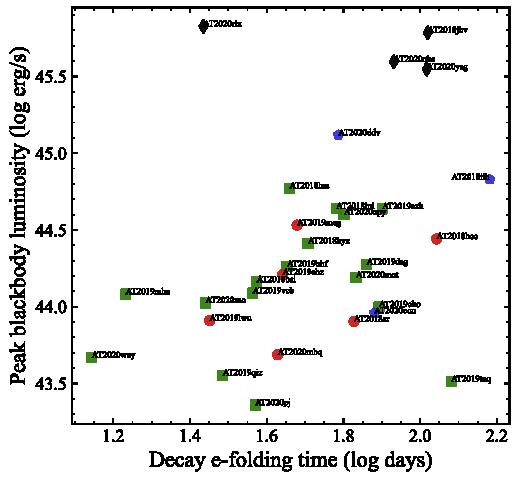
\includegraphics{nuclear/tde_bb_lumi_spread.pdf}
    \caption[TDE Blackbody luminosity spread]{TDE blackbody luminosity spread. Relevant is the y-axis here, showing the large spread in observed TDE luminosities; the TDEs shown are from the ZTF Phase I. From~\cite{Hammerstein2022}}
    \labfig{bb_lumi_spread}
\end{marginfigure}

This model has been realized as an instantiation of an \texttt{SNCosmo} source model, as this package has the advantage of built in filter profiles, that allowed the correct evaluation of the blackbody flux as seen through the ZTF filters. To save computing time, the fit algorithm used was not a Markov-Chain Monte Carlo as in~\cite{Velzen2021a}, but \texttt{iminuit/MIGRAD}.

To account for Milky Way dust extinction along the line of sight, the infrared dust maps by Schlegel, Finkbeiner y \& Davis were used~\sidecite{Schlegel1998}, as provided by the \texttt{sfdmap}\sidenote{\url{https://github.com/kbarbary/sfdmap}} Python package.

\subsubsection{TDE Fit Priors}
To constrain the fits and mitigate runaway, fit priors were used, partly taken from~\cite{Velzen2021a}. These are shown in Table~\ref{tab:tde_fit_priors}.

The prior on the time of peak, here dubbed $t_0$, was inferred from a peak finding algorithm that identified the highest flux point in each band (given it had a signal-to-noise ratio of $>3$) after smoothing the light curve with a rolling window, calculating the median flux within a widow width of 10 days.

\begin{table}[h]
    \begin{center}
        \begin{tabular}{c|c|c|c}
            Param.               & Description        & Prior    & Bounds                              \\
            \hline
            $t_\text{peak}$      & Peak time          & $t_0$    & $t­_0 \pm 30$ days                  \\
            $\log T_\text{peak}$ & Peak temperature   & 4 K      & [3.5, 5]~\unit{\K}                  \\
            $\log \sigma$        & Gaussian rise time & 1.6 days & [0,5] days                          \\
            $\log \tau$          & Exp. decay time    & 2.3 days & [0,5] days                          \\
            $\Delta T$           & Temp. change / day & 0        & $T_\text{peak} \pm 15000$ K (total) \\
            $t_\text{cutoff}$    & End of temp. evol. & 300      & [100, 1200] days $+t_0$
        \end{tabular}
    \end{center}
    \caption[TDE Fit priors]{Priors for the TDE fit.}\label{tab:tde_fit_priors}
\end{table}

As the blackbody fits were not constrained by UV data, in some cases \textbf{temperature runaway} occured when allowing all fit parameters to vary freely within their bounds. This can be explained as follows: A decrease in brightness over time can be either be achieved by exponential decay or by an increase in temperature. The latter gradually moves the blackbody spectrum outside the ZTF bands, which then translates to decreasing brightness. As such excessive temperature changes are most likely unphysical, the daily temperature change $\Delta T$ was limited to an integrated maximum change of $T_\text{peak} \pm \SI{1.5e4}{\K}$.

Another measure to mitigate the issue was to perform the fits as a \textbf{two-stage process}: First, the temperature evolution was disabled, i.e. $\Delta aT$ was set to $0$ and $t_\text{cutoff}$ was removed as parameter, with the blackbody only having one temperature for the duration of the light curve, $T_\text{peak}$. The best-fit values for $t_\text{peak}$, $\log T­­_\text{peak}$, $\log \sigma$ and $\log \tau$ obtained in this first stage were then used as fit priors for stage 2. This procedure solved the temperature runaway in almost all cases.

\begin{figure}[htb]
    \centering
    \begin{subfigure}[b]{0.49\textwidth}
        \centering
        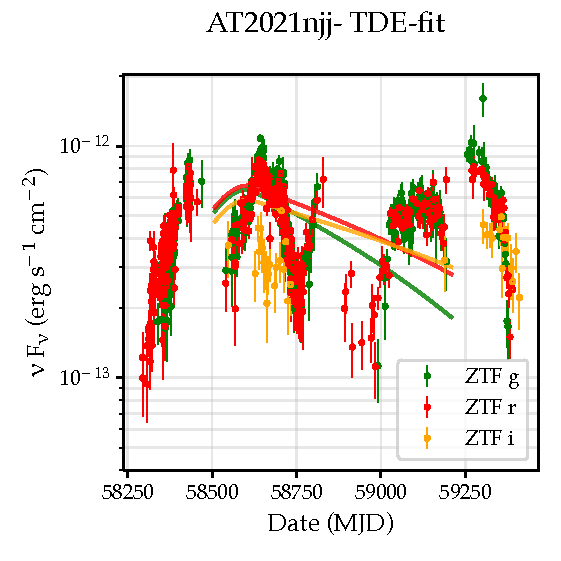
\includegraphics[width=1\textwidth]{nuclear/ZTF18aaymybb_exp.pdf}
    \end{subfigure}
    \begin{subfigure}[b]{0.49\textwidth}
        \centering
        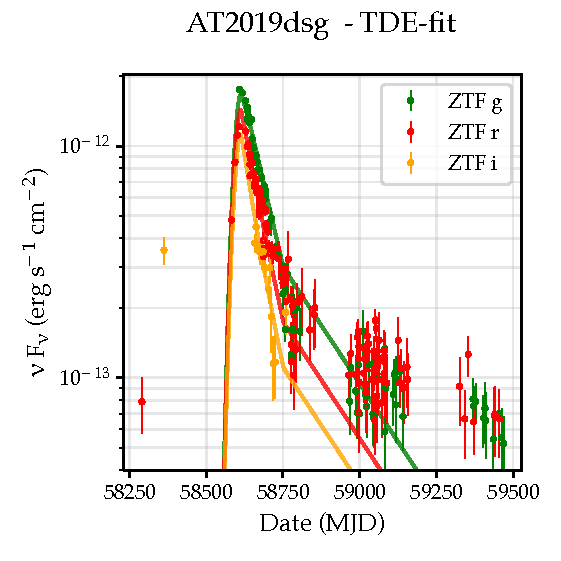
\includegraphics[width=1\textwidth]{nuclear/ZTF19aapreis_exp.pdf}
    \end{subfigure}
    \caption[Two exemplary TDE fits]{Two exemplary TDE light curve fits. \textbf{Left}: \textit{AT2021njj}, displaying periodic AGN activity not well captured by the fit.\ \textbf{Right}: \textit{AT2019dsg}, a TDE which is captured fairly well by the fit routine.}
    \labfig{tde_fit_comparison}
\end{figure}

Fig.~\ref{fig:tde_fit_comparison} shows \textbf{two exemplary TDE fits}; one for an object of unknown nature (\textit{AT2021njj}) on the left and one for a confirmed TDE (\textit{AT2019dsg}, see Section \ref{at2019dsg}) on the right. As one can see, the fit captures the light curve evolution of the TDE fairly well, including the change in color due to the changing blackbody temperature.~\textit{AT2021njj} on the other hand --- whatever it actually is, as the object has no spectroscopic classification except for `AGN', it is clearly not a TDE. The fit unsurprisingly cannot account for the periodic nature of the object, resulting in a reduced $\chi^2$ of $26.3$.

The successful fit for \textit{AT2019dsg} meanwhile results in the following values: A reduced $\chi^2$of $4.1$, a peak temperature of \SI{8700}{\K} which decays by \SI{78}{\K} per day for the following 138 days, an initial risetime of 21 days, and a characteristic light curve decay time of 216 days.

This object nevertheless highlights a restriction: The available optical to infrared data from ZTF does not constrain blackbodies well. When including additional UV data for \textit{AT2019dsg} near light curve maximum, the inferred blackbody temperature is \SI{4e4}{\K}, significantly higher. This is not a failure of the fit procedure, but driven by the high UV flux (which can be seen in Fig.~\ref{fig:at2019dsg_lc}).

\subsection{Fitting a SN Ia Model}
As \textbf{SNe Ia are a prominent contaminant} for bona fide nuclear events (i.e.~such events that can only occur in the centers of galaxies), it is crucial to identify them. To achieve this goal, all light curves were additionally subjected to a fit using the tried and tested Spectral Adaptive Lightcurve Template (SALT2)~\sidecite{Guy2007} light curve model.

SALT2 assumes the light curve is indeed a supernova Ia and applies empirical corrections to the light curve color and stretch (i.e.~the width of the light curve). This is achieved by matching templates generated by a set of well-sampled Ia light curves and spectra of varying distance. The resulting color and stretch correction parameters, as well as the peak brightness and the reduced $\chi^2$ were saved and will later be used as features in training a machine learning model.

\begin{figure}[H]
    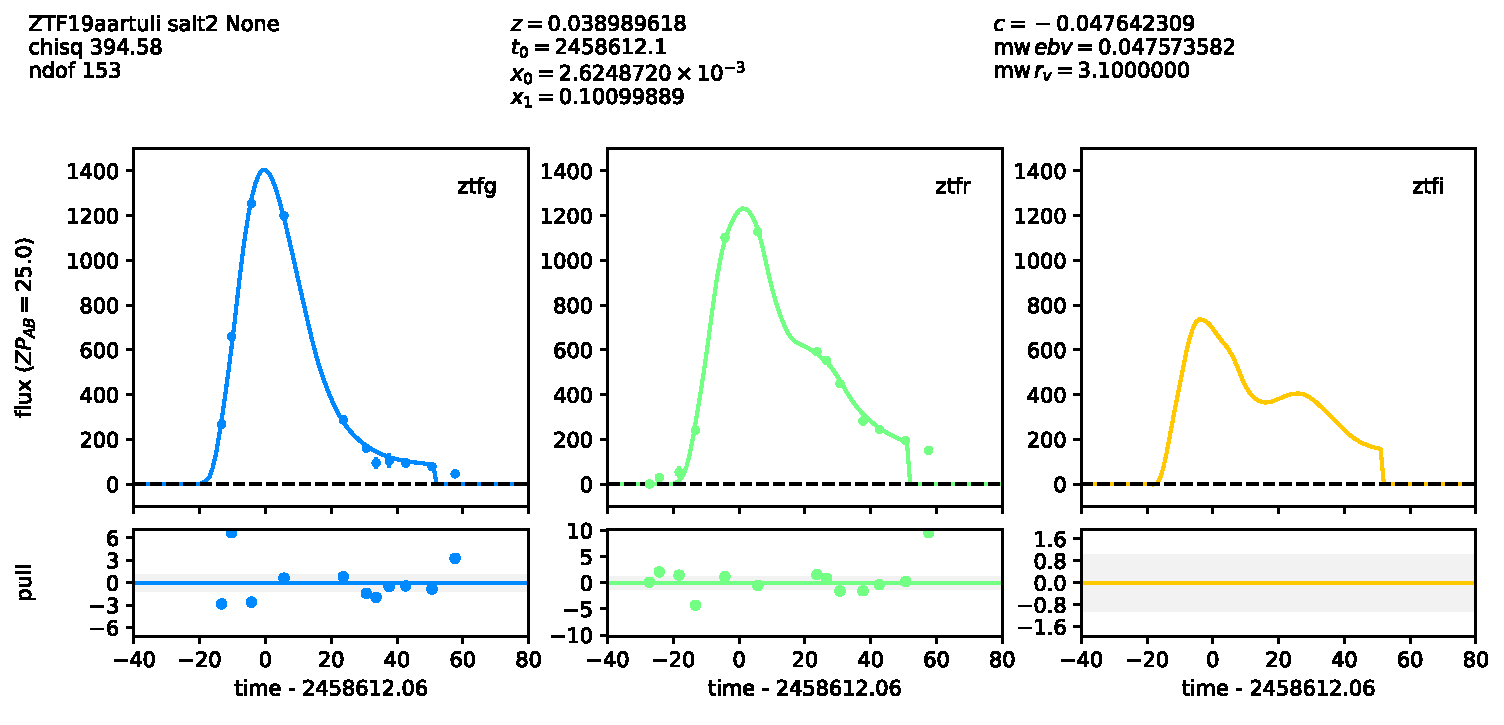
\includegraphics[width=1\textwidth]{nuclear/salt.pdf}
    \caption[SALT2 Fit]{Examplary SALT2 fit output. The three panels show three ZTF bands. Time 0 is the fitted peak of the assumed SN Ia; and as one can see the transient in question is fairly well approximated by SN Ia light curve, with a reduced  $\chi^2=2.67$. The transient is in a fact a spectroscopically classified supernova Ia.}
    \labfig{salt2}
\end{figure}

The fits were performed with \texttt{SNCosmo}, which itself fit the light curve using \texttt{iminuit/MIGRAD}.

\section{Optical Flare Analysis}
Another feature which will later be used in the classification of transients are \textbf{simultaneous flares} across the well-sampled ZTF \textit{g}- and \textit{r}-bands. The number and timing of optical flares within different bands can then be used to differentiate between different types of transients.

\subsection{Bayesian Block Algorithm}
To determine time periods of heightened activity, a Bayesian block algorithm was employed. This was a version of a package developed at DESY, modified by the author to analyze optical ZTF light curves instead of infrared \textit{WISE} data.

The Baysian Block algorithm is explained in~\sidecite{Scargle1998}; the implementation used here is integrated in the \texttt{astropy} package. The light curves are first smoothed by calculating the median and standard deviation within a 10 day rolling window. After that, only data points lying within $3 \sigma$ distance in magnitude space from the median are used. This gets rid of flux outliers, which are quite frequent for the forced photometry light curves of the nuclear sample.

The prior used for the Bayesian Block analysis was $10 \times \log(n_\text{data})$, with $n_\text{data}$ being the number of datapoints in the smoothed single-band light curve. These numbers were determined empirically to yield robust results. They are a compromise between sensitivity to flux changes and detecting too many, too small blocks to be meaningful.

\subsection{Block Coincidence}
As they are much better sampled than the \textit{i}-band, the \textit{g}- and \textit{r}-band are used to check for blocks temporally coincident in both bands.

For this, each region with increased flux compared to a baseline in the \textit{g}-band is checked to see if there is a corresponding \textit{r}-band block with increased flux overlapping in time.

\begin{figure}
    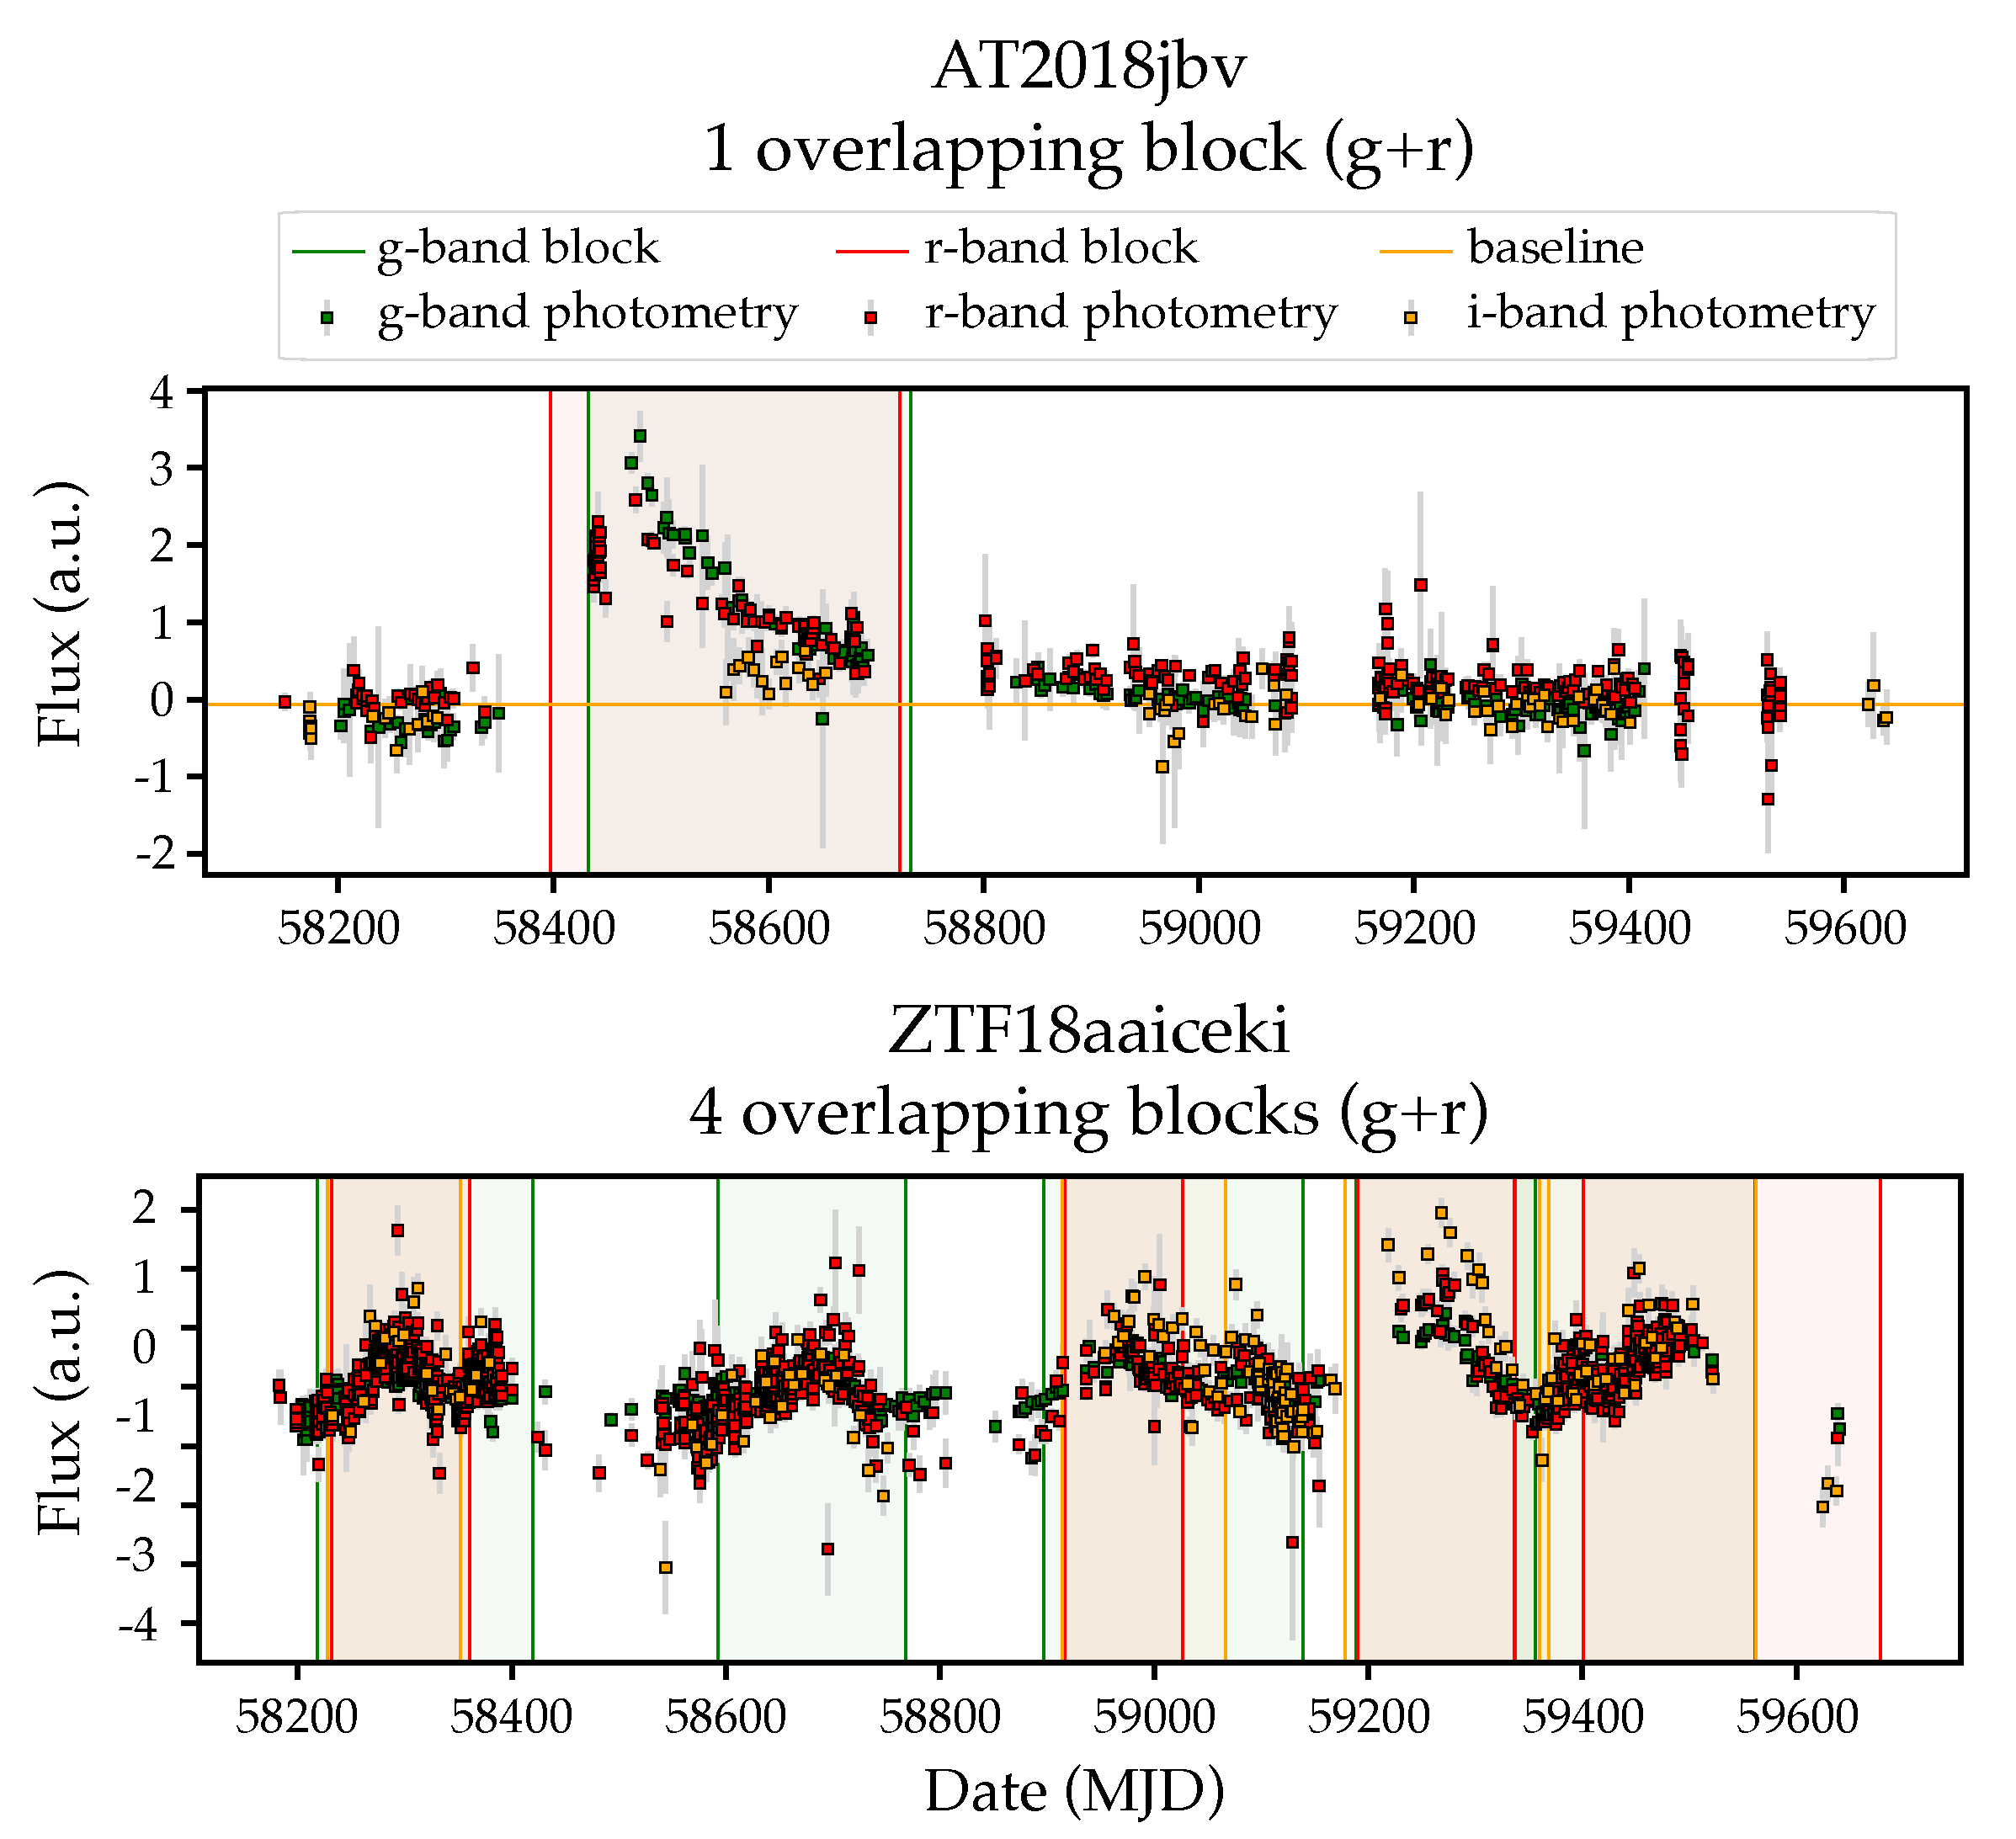
\includegraphics[width=1\textwidth]{nuclear/bayesian_blocks.pdf}
    \caption[Bayesian Blocks]{\textbf{Top}: Bayesian Blocks identified for \textit{AT2018jbv}. There is one block both in \textit{g}- and \textit{r}-band, which overlaps. This is a strong indicator that the transient is a one-time flare, stemming from e.g.~a supernova or a TDE (the transient is in fact a TDE), in contrast to stochastic AGN variability. \textit{Bottom}: Bayesian Blocks for ZTF18aaiceki, showing AGN activity. This is correctly captured by a large number of overlapping regions.}
    \labfig{bayesian_blocks}
\end{figure}

One can see two examples of such overlapping blocks in Fig.~\ref{fig:bayesian_blocks}, which shows the result of the Bayesian Block algorithm for \textit{AT2018jbv} and \textit{ZTF18aaiceki}. Both are transients from the nuclear sample, the first one being a TDE, the second an AGN displaying stochastic variability.

\section{Training Sample}
As one of the goals is the machine-based classification of the nuclear sample, a training sample that most closely resembles the target sample --- the nuclear sample --- in brightness.

\subsection{The Bright Transient Survey}
The natural starting point for the creation of a training sample was the so-called ZTF Bright Transient Survey (BTS)\sidenote{\url{https://sites.astro.caltech.edu/ztf/bts/bts.php}}, see~\cite{Fremling2020,Perley2020} for details. The basic goal of the survey was spectroscopic classification of all ZTF-detected transients brighter than 18.5 mag in either the \textit{g}- or \textit{r}-band. It even pushes further, achieving a spectroscopic completeness of \SI{75}{\percent} at 19 mag (\SI{93}{\percent} at the nominal cutoff of 18.5 mag)~\cite{Perley2020}.

This was achieved by utilizing the fully robotic SED machine for quick classification, and employing other spectroscopic resources for ambiguous results. BTS is the largest spectroscopic supernova survey ever conducted, with over 8000 classified transients so far (August 2023).

There are three potential issues that need to adressed though when using the BTS as starting point for a training sample:

\begin{description}
    \item[Brightness bias] The BTS restriction to objects usually brighter than 18.5 mag means that the majority of the BTS sample will be brighter than the nuclear sample with its magnitude cut of 20.
    \item[Class imbalance] The BTS is heavily skewed towards supernovae. Also, because SNe Ia are brighter, the majority of the SNe contained in a flux-limited sample like the BTS will be of Type Ia. Roughly 3/4 of all BTS transients are SNe Ia~\cite{Perley2020}.
    \item[Anti-AGN bias] To reduce contamination stemming from AGN variability, the BTS vetoes transient host galaxies that likely harbor an AGN. This is achieved by crossmatching candidate sources to known AGN, based on \textit{WISE} color cuts, or by rejecting sources with previous variability most likely hinting at AGN activity. As the nuclear sample will contain
\end{description}

These issues need to be solved somehow. Two procedures will be described below: \textbf{Noisification} addresses the brightness bias and partially the class imbalance, while \textbf{either rejecting likely AGN} within the nuclear sample or \textbf{expanding the training set} with known AGN deals with the anti-AGN bias.

\subsection{Noisification: Enhancing the training set}
One promising strategy is to multiply the number of light curves available by simulating observations of the same object at higher redshifts.

This method, here dubbed ``Noisification'', was developed by Alice Townsend, with significant contribution by the author. The procedure works as follows:

Obtain a transient light curve (from now on: parent light curve) and parent redshift $z_\text{parent}$ (all classified BTS transients have a spectroscopic redshift). \textbf{Draw a new redshift} $z_\text{child}$ for the child light curve (i.e. the noisified copy) from a cubic redshift distribution ranging from $z­_\text{parent}$ to $z_\text{parent}+0.1$.

After this, \textbf{the parent flux was redrawn} from a normal distribution centered around each parent flux value, scaled by its error. This was done to account for the fact that flux measurements are expected to scatter around their true value with their error, thereby simulating a `new' measurement. After this, the re-drawn flux measurements were rescaled with the new redshift $z_\text{child}$. The flux $F$ scales according to $D_L=\frac{L}{4 \pi F}$ i.e.~with the square of the luminosity distance (see Section~\ref{fitmodels}). Therefore, one can determine a \textbf{flux scaling factor} $a$ according to
\begin{equation}
    a = \frac{D_L(z_\text{parent})^2}{D_L(z_\text{child})^2}.
\end{equation}
With this scaling factor, the child lightcurve flux is simply $f_\text{child} = a f_\text{parent}$.

If an \texttt{SNCosmo} model for the transient type did exist, \textbf{K-correction} was applied. This procedure accounts for the fact that by arbitrarily redshifting the light curve of an object, the spectrum will also be redshifted. Due to this, the bandpasses will register different parts of the spectrum, which leads to a different observed flux (see~\sidecite{Hogg2002} for an introduction).

If

\subsection{AGN Rejection}

\subsection{Sample Enhancement}